\begin{multicols}{3}[\section{NFC}]

\rhead{Autor: Mirko Grothe}
\lfoot{Letzte Bearbeitung: 16.04.2016}

\newrefsegment

\begin{boxedminipage}{\linewidth}
\begin{tabular}{p{2,1 cm}p{2.7 cm}}
\textbf{Steckbrief}& \\
\end{tabular}
\begin{tabular}{p{2,1 cm}|p{2.7 cm}}
      Einsatz seit & 2002\\
      \hline
      Frequenz"-bereich  & \SI{13.56}{\mega\hertz}\\
      \hline
      Datenrate & \SI{424}{kBit/s}\\
      \hline
      Verbreitung & gering\\
      \hline
      Reichweite & \SI{4}{cm}\\
\end{tabular}
\end{boxedminipage}
\par


\subsection*{Überblick}
Near Field Communication (z.dt. Nahfeldkommunikation, Abkürzung NFC) ist ein internationaler Übertragungsstandard zum kontaktlosen Austausch von Daten zwischen zwei Geräten. NFC wurde 2002 von Philips und Sony entwickelt und wird seit 2004 durch das NFC-Forum spezifiziert. Die Übermittlung funktioniert über eine Distanz von bis zu 4 Zentimetern und ist mit einer maximalen Übertragungsrate von 424 kBit/s nicht für das Senden umfangreicher Daten wie Bildern oder Videos geeignet. Stattdessen ist NFC auf Dienste ausgelegt, bei denen ein Transfer geringer Datenmengen über kurze Reichweiten initiiert wird, ohne das bei jedem Verbindungsaufbau eine zeitintensive Kopplung erforderlich ist. Typische Einsatzgebiete sind bargeldloses Zahlen und digitale Tickets und Schlüssel.
Die Datenübertragung ist intuitiv und kann daher bei entsprechender Konfiguration automatisch gestartet werden, sobald ein NFC-fähiges Gerät in Reichweite ist.~\cite{nfc.1,nfc.2,nfc.12}

\begin{Figure}
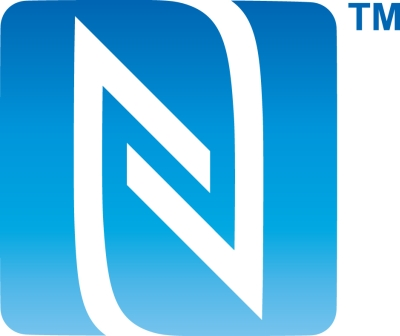
\includegraphics[width=\linewidth]{Kapitel/NFC/Grafiken/Logo.jpg}
\captionof{figure}{N-Mark-Logo als Kennzeichnung NFC-zertifizierter Geräte~\cite{nfc.1}}
\label{fig:nfc.logo}
\end{Figure}

\subsection*{Technische Erläuterungen}
NFC wurde gezielt für eine Übertragung geringer Datenmengen mit schnellem Verbindungsauf und -abbau entwickelt. Dies wird realisiert, indem der Daten-Transfer zwischen zwei NFC-fähigen Geräten automatisch initiiert wird, sobald diese in Reichweite sind. Um unbeabsichtigte Verbindungen oder ein Abhören der zu übermittelnden Daten zu verhindern, ist die Übertragung mit NFC nur in geringer Reichweite im Zentimeterbereich möglich. Damit kann eine Kontaktaufnahme als Zustimmung zu einer Daten-Transaktion gewertet werden. Bei sicherheitskritischen Transaktionen wie Kreditkarten-Zahlungen erfolgt die Kommunikation zusätzlich verschlüsselt.

Jedes NFC-Gerät unterstützt zwei Betriebsmodi. Im passiven Modus wird das Senden und Empfangen von Daten von einem anderen aktiven Gerät initiiert und gesteuert. Das passive Gerät kann hierbei ausgeschaltet sein. Im aktiven Modus kann ein Gerät zusätzlich zur passiven Funktion einen Datentransfer selbst veranlassen. Sind beide Geräte im aktiven Modus, so spricht man auch vom sogenannten Peer-to-Peer-Modus, da ein Datenaustausch in Form eines Dialogs möglich ist. Des Weiteren gibt es sogenannte NFC-Tags; diese besitzen im Gegensatz zu NFC-Geräten keine eigene Stromversorgung und können äquivalent zu ausgeschalteten Geräten nur im passiven Modus arbeiten. Darüber hinaus können sie, anders als NFC-Geräte, nicht gleichzeitig Daten senden und empfangen.

NFC nutzt die RFID-Technologie (radio-frequency identification), ein Sender-Empfänger-System zum automatischen und berührungslosen Identifizieren von Objekten über Funkwellen mit einer Frequenz von 13.56~MHz~\cite{nfc.9}. Jedes NFC-Gerät (nicht NFC-Tags) kann sowohl die Rolle des Senders, als auch die des Empfängers übernehmen. Mit seiner Peer-to-Peer-Funktion grenzt sich NFC zur RFID-Technologie ab, bei der nur eine Kommunikation zwischen aktivem Sender und passivem Empfänger möglich ist. Die Kommunikation über NFC wird durch den internationalen Übertragungsstandard ISO/IEC 18000-3 spezifiziert.

Ein anfragendes Gerät erzeugt mittels einer Spule ein elektromagnetisches Wechselfeld mit einer Trägerfrequenz von 13,56~MHz. Unterschreitet es dabei den maximalen Sende-Radius zu einem anderen Gerät, so induziert es über eine Spule im Stromkreis des empfangenden Gerätes eine Spannung. Weil das Magnetfeld aufgrund der Wechselspannung nicht konstant ist, fungiert es für das empfangende Gerät als konstante Energie-Quelle, solange letzteres sich innerhalb dessen Sende-Reichweite befindet. Aus diesem Grund kann ein Gerät im passiven Modus ausgeschaltet, also von seiner eigenen Energieversorgung getrennt sein und ein NFC-Tag ohne eigene Energiequelle auskommen.

Über die sogenannte induktive Kopplung zwei benachbarter elektrischer Stromkreise erfolgt neben der Energieübertragung auch die Kommunikation der beiden Geräte. Die Daten werden über das Magnetfeld per Phasen-Jitter-Modulation (PJM) von dem anfragenden Gerät an das empfangende Gerät gesendet. Die PJM ist eine abgeschwächte Form der Phasenmodulation, bei der vom sendenden Gerät nur sehr kleine Änderungen an der Phase des Trägersignals vorgenommen werden. Während der unmodulierte Teil des Signals zur Energieversorgung des Empfängers dient, demoduliert und interpretiert dieser den geringen modulierten Anteil des Signals durch Vergleichen mit dem unmodulierten Anteil. Bei der Datenübertragung vom Empfänger zurück zum anfragenden Gerät bedient sich Ersterer der modulierten Rückstreuung. Hierbei reflektiert der Empfänger das empfangene Signal mit gleicher Trägerfrequenz und gleichzeitig veränderten Amplituden (Amplituden-Modulation). Dies wird durch kurzeitiges Ändern der Impedanz (Widerstand) der Empfänger-Spule realisiert. Durch Demodulation und Interpretation der veränderten Amplituden des zurückgestreuten Signals erhält das anfragende Gerät die Antwort des empfangenden Gerätes.
 
Die Übertragung der Daten kann entweder verbindungslos oder verbindungs-orientiert erfolgen, wobei NFC-Tags und Geräte im passiven Modus auf die verbindunglose Datenübertragung beschränkt sind. Bei sicherheitskritischen Transaktionen wie Kreditkarten-Zahlungen wird grundsätzlich eine verbindungs-orientierte Datenübertragung verwendet.~\cite{nfc.3,nfc.4,nfc.5,nfc.6,nfc.7,nfc.8}


\subsection*{Einsatz}
NFC wurde zur kontaktlosen Datenübertragung über kurze Distanzen entwickelt. Damit konkurriert NFC nicht mit Funkstandards wie Bluetooth oder WIFI, welche höhere Übertragungsraten und Reichweiten bieten, sondern stellt eine Alternative zu Datenübertragungen mit physischer Schnittstelle dar. Aufgrund des schnellen Verbindungsauf- und –abbaus hat NFC das Potenzial, Kreditkarten und Schlüssel abzulösen; denn im Gegensatz zu den herkömmlichen Datenübertragungs- und Autorisierungs-Technologien entsteht bei der Verwendung von NFC kein physischer Verschleiß an den Geräten. Zudem sind dadurch wasserdichte Konstruktionen der Geräte möglich.
Anwendung von NFC findet sich im Mobile-Payment zum kontaktlosen Bezahlen mit NFC-fähigen Kreditkarten oder Smartphones. Eine größere Verbreitung hat NFC allerdings im Bereich der Autorisierung. Typische Einsatzgebiete sind Schlüsselkarten zum Öffnen von Türen und Schranken, digitale Eintritts- und Fahrkarten, und Chips zur Arbeitszeit-Erfassung durch sogenanntes „Einchecken“. In Schlüsselkarten werden allerdings häufig noch RFID-Chips verwendet. Des Weiteren wird NFC häufig zum automatischen Pairing zweier Geräte über Bluetooth verwendet. Indem die zum Aufbau der Bluetooth-Verbindung benötigten Daten per NFC übertragen werden, kann der eigentlich langsame Verbindungsaufbau über Bluetooth zwischen zwei Geräten überbrückt werden.~\cite{nfc.1,nfc.2,nfc.10}

\begin{Figure}
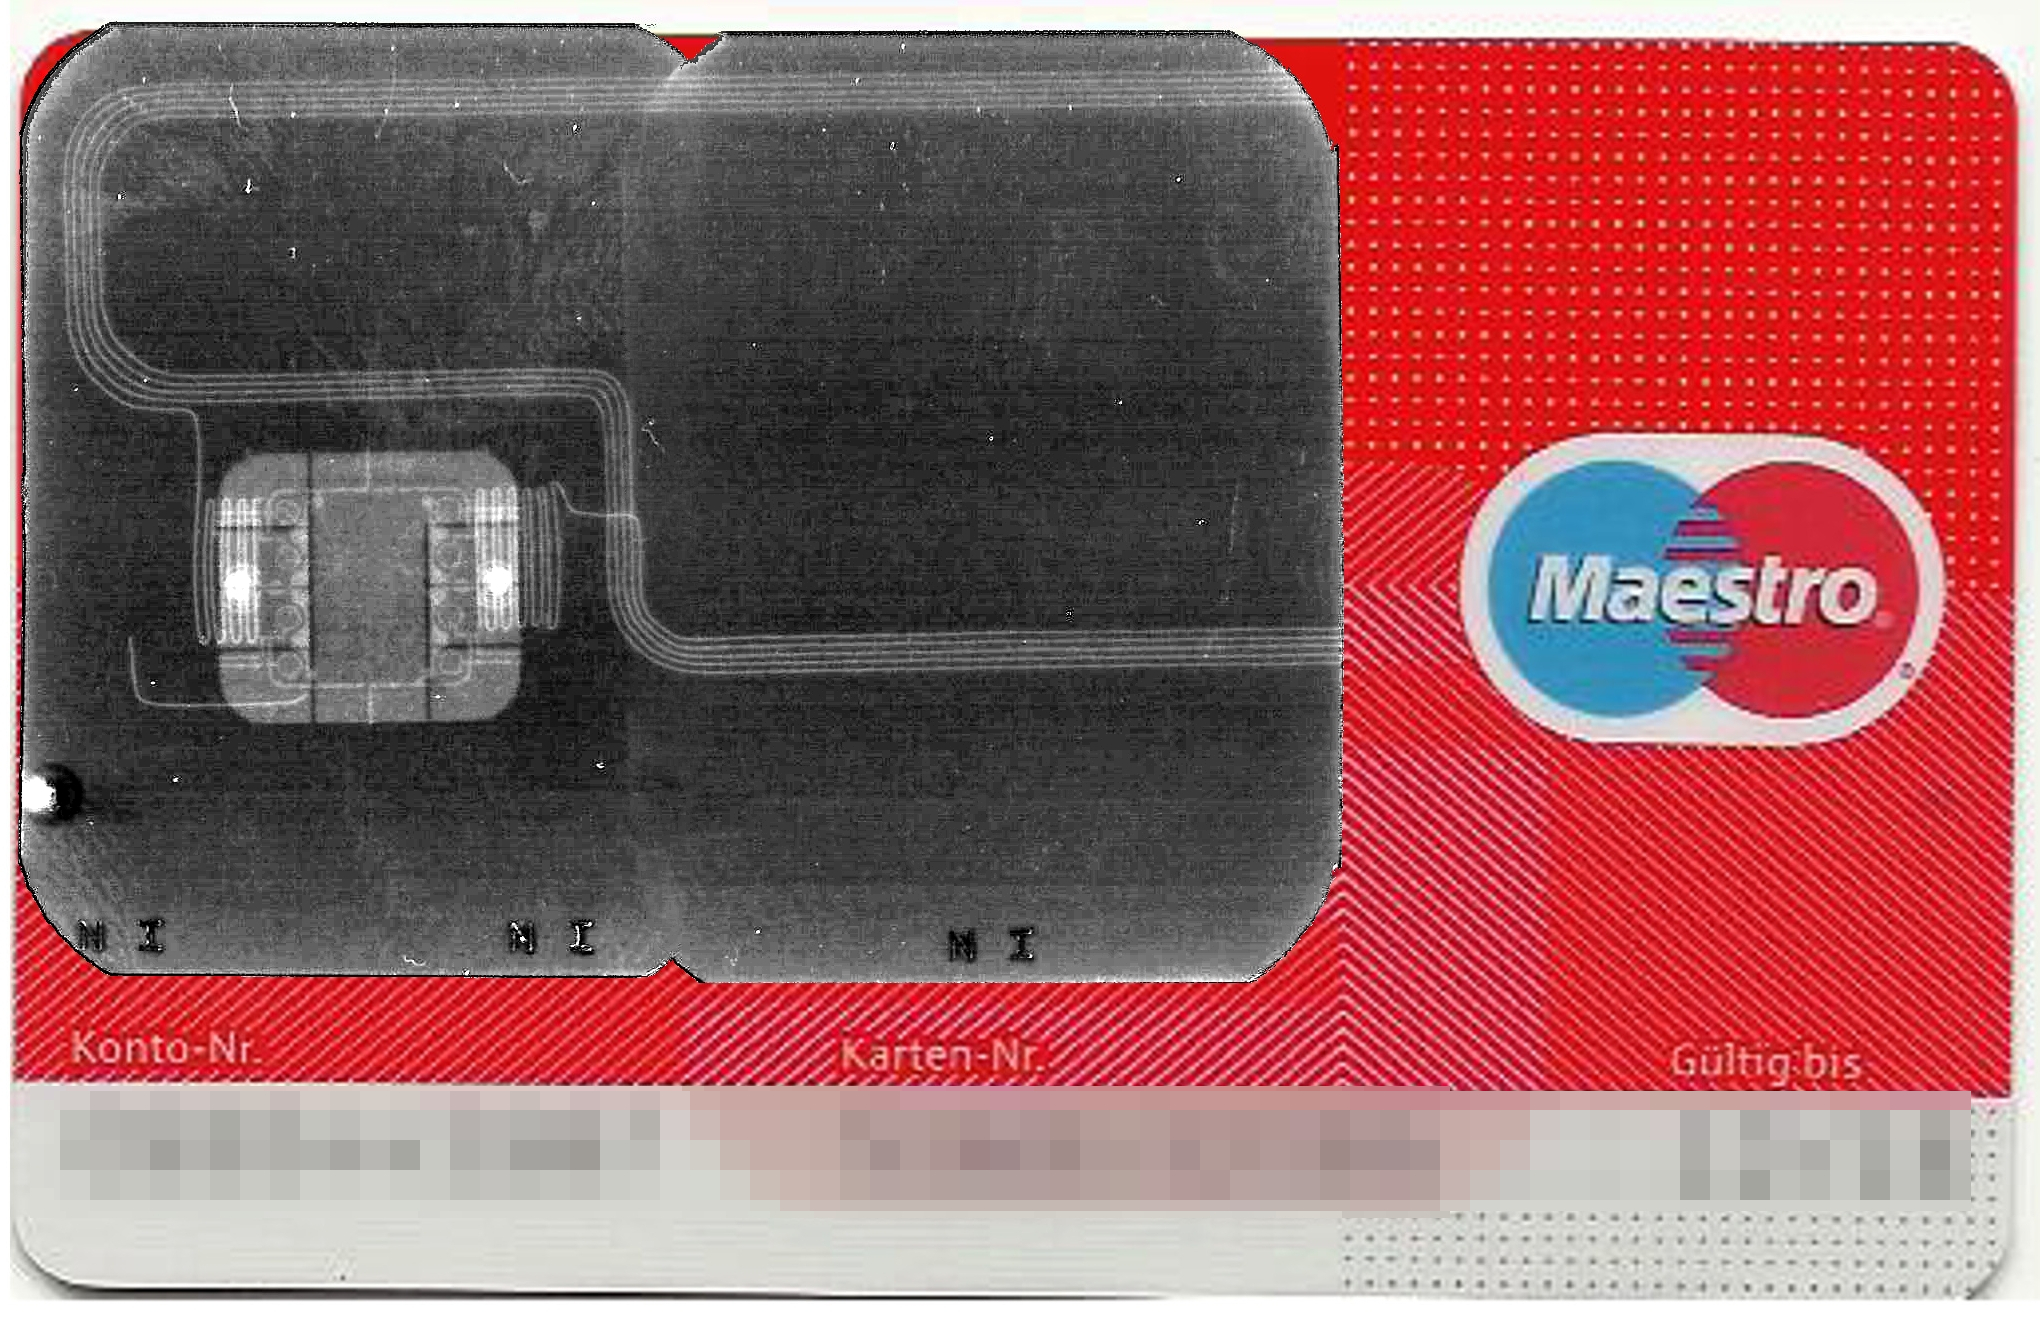
\includegraphics[width=\linewidth]{Kapitel/NFC/Grafiken/girogo.jpg}
\captionof{figure}{Röntgenansicht der girogo-Karte~\cite{nfc.1}}
\label{fig:nfc.girogo}
\end{Figure}


\end{multicols}
\newpage
\section*{Historische Entwicklung~\cite{nfc.1}}
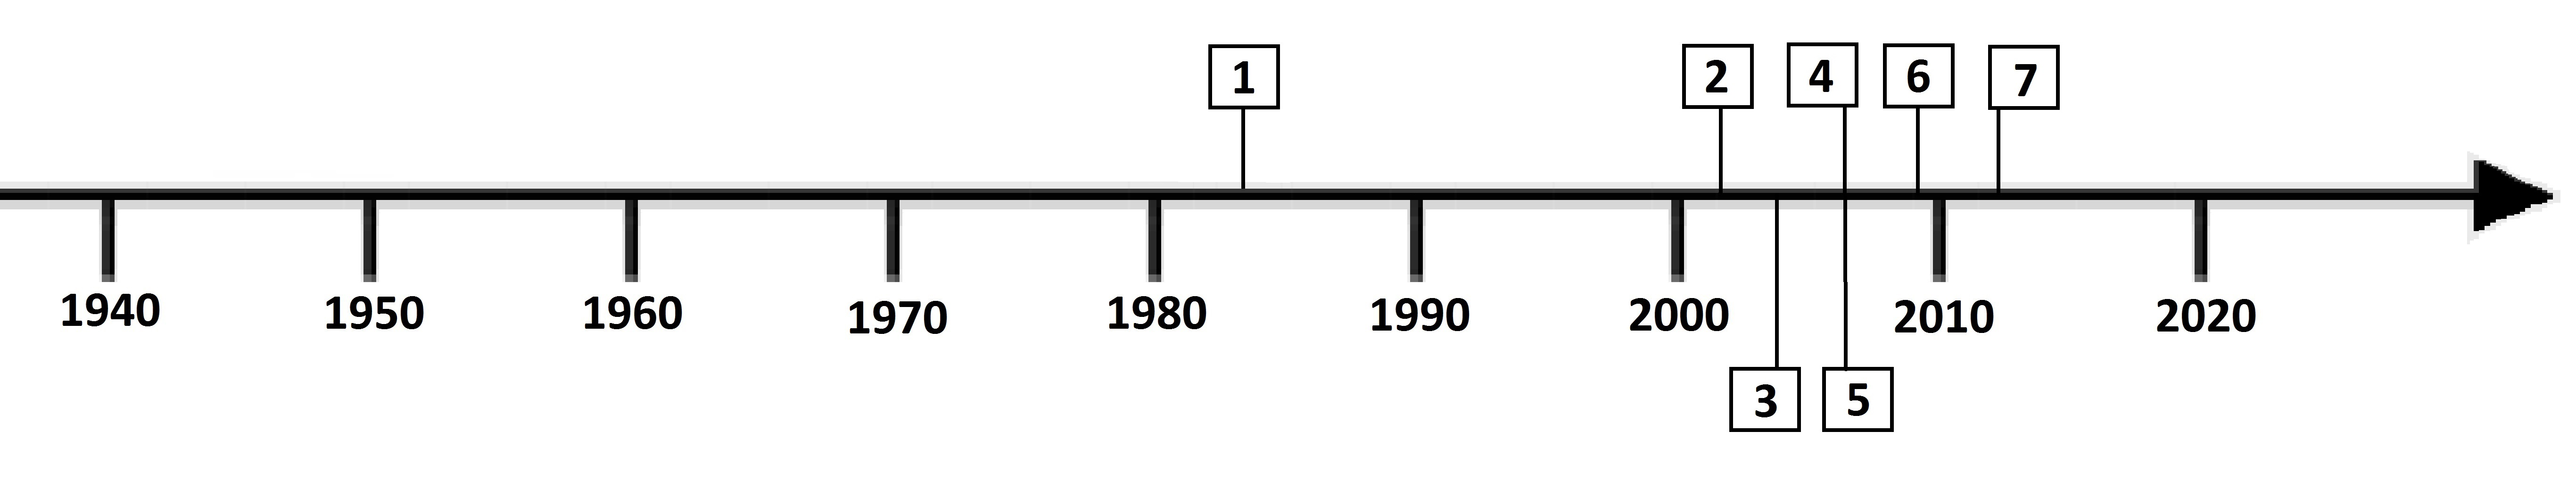
\includegraphics[width=\textwidth]{Kapitel/NFC/Grafiken/Zeitstrahl}
\par
\noindent
\begin{tabular}{|p{1 cm}|p{3 cm}|p{13.55 cm}|}
	\hline
	Nummer & Datum & Entwicklungsschritte\\
	\hline
	1 & 1983 & Das erste Patent mit der Abkürzung „RFID“ wird auf Charles Walton ausgestellt.\\
	\hline
	2 & 2002 & Sony und Philips einigen sich auf eine technische Spezifikation.\\
	\hline
	3 & 2004 & Nokia, Philips und Sony etablieren das Near Field Communication (NFC) Forum.\\
	\hline
	4 & 2006 & Erste Spezifikation für NFC-Tags wird veröffentlicht.\\
	\hline
	5 & 2006 & Nokia präsentiert das erste NFC-fähige Mobiltelefon.\\
	\hline
	6 & 2009 & Das NFC-Forum veröffentlicht Peer-to-Peer-Standards.\\
	\hline
	7 & 2012 & Einführung von girogo.\\
	\hline
\end{tabular}
\par
\begin{multicols}{3}

\subsection*{Anbieter und Gremien}
Die 2002 von Philips und Sony entwickelte Nahfeldkommunikation wird durch die öffentliche Plattform NFC-Forum spezifiziert. Die Spezifikationen umfassen Standards für die Gerätearchitektur von NFC-Geräten und die bei der Kommunikation verwendeten Protokolle.

NFC als Autorisierungs-Tool findet in Unternehmen Anwendung im Öffnen von Türen und Schranken. Die NFC-Tags können für jeden Mitarbeiter entsprechend seiner Rolle konfiguriert werden und so jedem die individuell benötigten Zugangsrechte verschafft werden. Über den Schlüssel-Ersatz hinaus, der auch mit herkömmlichen RFID-Chips möglich ist, können NFC-Chips aufgrund ihrer Peer-to-Peer-Funktion von Unternehmen zur Arbeitszeit-Erfassung ihrer Mitarbeiter verwendet.

Seit Anfang 2012 haben in Deutschland Kreditkarten von Visa (payWave) und MasterCard (PayPass) einen NFC-Chip verbaut. Damit können bei kooperierenden Händlern Beträge bis maximal 25 Euro ohne PIN-Abfrage bezahlt werden. Sparkassen und Volksbanken bieten mit ihrer Girocard (girogo (Abbildung~\ref{fig:nfc.girogo})) ebenfalls eine NFC-Funktion zum kontaktlosen Bezahlen.
Studenten-Ausweise mit denen man kontaktlos bezahlen kann und auch der neue Personalausweis enthalten in der Regel noch RFID- statt NFC-Chips.

Bei modernen Multimedia-Systemen ist NFC häufig bei Vorhandensein einer Bluetooth-Funktion anzutreffen, um ein schnelles und kontaktloses Pairing mit einem anderen Bluetooth-Gerät zu ermöglichen.~\cite{nfc.2,nfc.11,nfc.12}


\subsection*{Ausblick}
Als Studentenausweis mit Bezahl-Funktion oder Schlüssel-Ersatz für Mitarbeiter hat sich NFC bis heute nicht durchgesetzt, da hier die ältere RFID-Technologie bereits weit verbreitet im Einsatz ist. Während der Übertragungsstandard im Mobile Payment mit Anbietern wie Google Wallet noch ein Nischendasein fristet, bieten die neuen Kreditkarten von Visa (payWave) und MasterCard (PayPass) bereits die Möglichkeit per NFC zu bezahlen. Bis dato unterstützen allerdings nur wenige Händler diese Zahlungsmöglichkeit.

In ferner Zukunft wird der Trend vermutlich in Richtung einer virtuelle Bankkarte gehen, die eine Applikation in einem NFC-fähigen Smartphone darstellt.~\cite{nfc.2}




\printbibliography[segment=10,heading=subbibliography]

\end{multicols}
\newpage